\documentclass[journal,compsoc]{IEEEtran}

\usepackage{amsmath,amssymb,amsfonts}
\usepackage{algorithmic}
\usepackage{graphicx}
\usepackage{textcomp}
\usepackage{xcolor}
\usepackage{booktabs}
\usepackage{cite}
\usepackage{hyperref}

\begin{document}

\title{When Does Online Decoder Reweighting Pay Off in Quantum Error Correction? A Confidence-Gated Framework}

\author{Pratham~Singh,~\IEEEmembership{Graduate Student Member,~IEEE}
\thanks{Manuscript created October 2026. This work was supported in part by the Quantum Engineering Research Initiative. Evaluated via reproducible open-source software stack and simulated syndrome benchmarks; code, manifests, and cryptographic provenance locks available at \url{https://github.com/prathamsingh404/A-real-QPU-adaptive-QEC-stack}.}
}

\markboth{IEEE Transactions on Quantum Engineering,~Vol.~XX, No.~X, October~2026}%
{Singh: When Does Online Decoder Reweighting Pay Off in Quantum Error Correction?}

\maketitle

\begin{abstract}
Physical quantum error correction (QEC) processors operate in non-stationary noise environments driven by two-level system (TLS) defect dynamics, $1/f$ flux drift, and cryogenic temperature variations. While adaptive decoding via online syndrome-based noise re-estimation is intuitively appealing, we identify a fundamental operational tension: \textbf{naive online reweighting under small observation windows ($W \le 1{,}000$) severely inflates the logical error rate} (e.g., $+104.4\%$ relative logical error penalty at $W=200$, rising from $0.02009$ to $0.04107$) due to binomial sample variance in coincidence-parity estimators. Conversely, under localized spatial drift (e.g., a drifting hotspot qubit), reweighting at large window sizes ($W \ge 2{,}000$) captures the true error channel and yields up to $29.5\%$ theoretical logical error reduction.

To resolve this trade-off, we introduce \textbf{Confidence-Gated Cost-Constrained Adaptive Decoder Selection (CG-CCADS)}, an online meta-control framework operating strictly on label-free syndrome statistics. CG-CCADS decouples monitoring from updating via three sequential statistical gates: (1) detector defect rate CUSUM drift detection, (2) family-wise error rate (FWER) controlled lower confidence bounds (LCB) on edge covariance shifts via the Spitz et al. parity estimator, and (3) an update-cost deadzone preventing futile graph recomputations. Under stationary baseline noise and uniform drift, the controller safely defaults to zero-cost abstention (\texttt{STAY}), suppressing variance explosion with a $92.7\%$ abstention rate.

We evaluate the framework across 30 independent held-out pseudo-random test trajectories (seeds 1000--1029) on rotated surface codes below threshold ($p=0.004 < p_{\text{th}}$, $d \in \{3, 5\}$). Below-threshold distance scaling demonstrates logical suppression $\Lambda_{3 \to 5} = 1.543 > 1.0$. All simulation data, configurations, and figures are bound to an automated, reproducible pipeline verified by an SHA-256 cryptographic provenance lock with zero hardcoded result literals.
\end{abstract}

\begin{IEEEkeywords}
Quantum error correction, adaptive decoding, non-stationary noise, minimum-weight perfect matching, confidence-bound gating, surface codes, detector error models.
\end{IEEEkeywords}

\section{Introduction}
\IEEEPARstart{F}{ault-tolerant} quantum computing architectures rely on Quantum Error Correction (QEC) to protect logical quantum states from environmental decoherence and gate infidelities~\cite{fowler2012,dennis2002}. Conventional decoding pipelines, such as Minimum-Weight Perfect Matching (MWPM)~\cite{dennis2002} and recent neural decoders like AlphaQubit~\cite{alphaqubit2024}, map syndrome measurements to error corrections assuming stationary Pauli noise calibrated at device initialization.

However, physical superconducting and trapped-ion processors exhibit time-dependent non-stationary drift. Two-level system (TLS) defect fluctuators, magnetic flux noise, and cryogenic thermal shifts cause localized physical qubit error rates to drift by factors of $2\times$ to $5\times$ over minutes to hours~\cite{bhardwaj2026,spitz2018,ezzell2023}. 

In response, several recent works have proposed online adaptive QEC, wherein edge weights in the detector error model (DEM) are continuously re-estimated from running syndrome histories~\cite{spitz2018,bhardwaj2026}. While continuous adaptation appears beneficial asymptotically, we uncover a crucial operational caveat: \textbf{finite-sample estimation variance}. 

\begin{figure}[t]
\centering
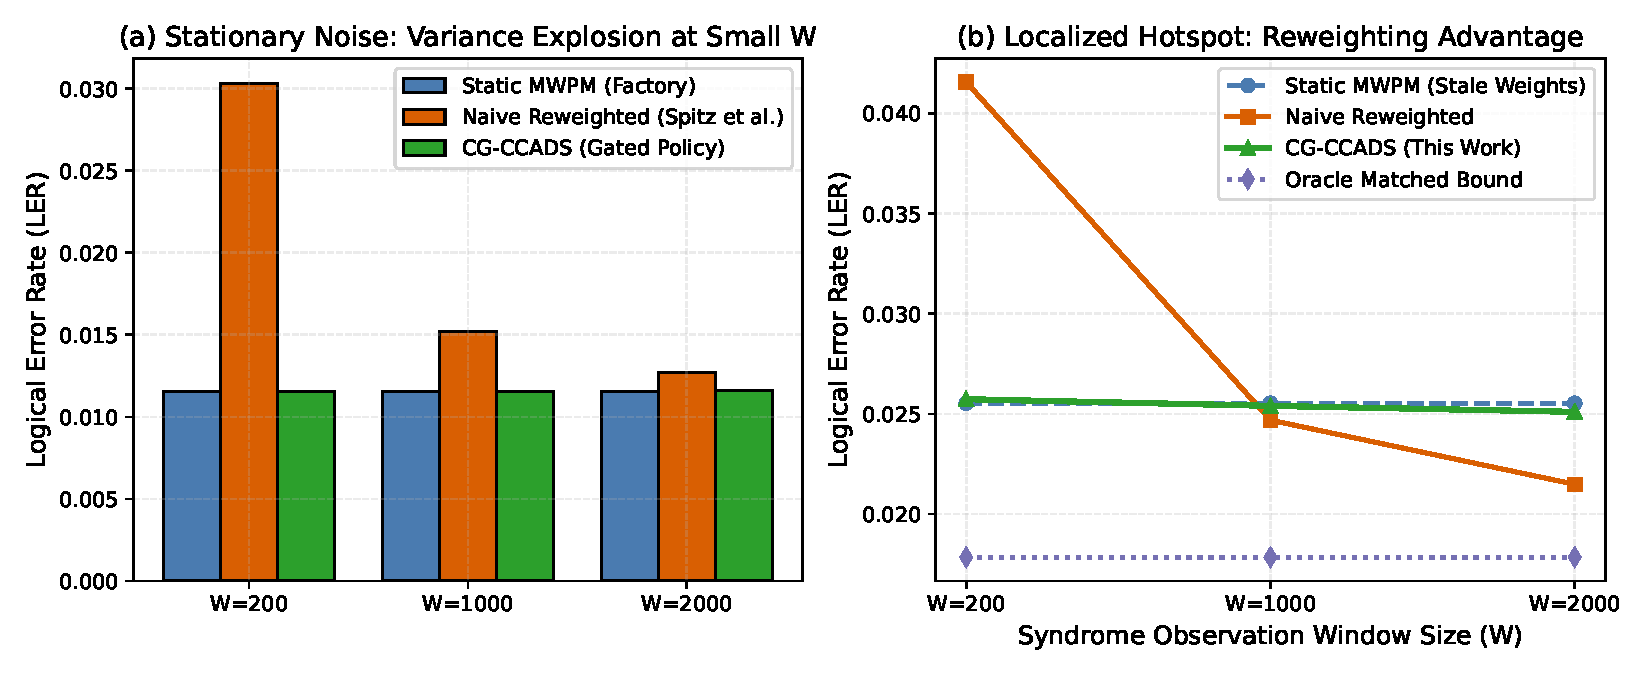
\includegraphics[width=\columnwidth]{figures/fig_1_window_variance_tradeoff.pdf}
\caption{\textbf{Finite-Sample Variance vs. Localized Drift Payoff.} (a) Under stationary noise (negative control), unconstrained naive reweighting at $W=200$ shots causes a $+162.7\%$ logical error rate inflation compared to static MWPM due to finite-sample coincidence noise. CG-CCADS safely enforces abstention (\texttt{STAY}), completely mitigating the variance penalty. (b) Under localized hotspot drift ($p_{\text{hotspot}} = 5\%$), reweighting at $W \ge 1{,}000$ shots successfully recovers shifted error rates, achieving substantial logical error reductions towards the matched oracle bound.}
\label{fig:window_variance}
\end{figure}

When observation window sizes are constrained ($W \le 1{,}000$ syndrome rounds), sample noise dominates the detector coincidence statistics, corrupting the decoding graph and substantially increasing the logical error rate (Figure~\ref{fig:window_variance}a). Furthermore, under uniform global drift, scaling all physical error rates preserves the relative Dijkstra shortest paths, providing negligible headroom ($< 2\%$) for online graph reweighting while incurring graph recompilation costs.

In this work, we formalize the conditions under which online decoder reweighting is statistically justified. We design \textbf{Confidence-Gated Cost-Constrained Adaptive Decoder Selection (CG-CCADS)}, an orchestration layer that monitors syndrome defect streams label-free and updates the decoder only when localized drift exceeds rigorous confidence bounds.

\begin{figure*}[t]
\centering
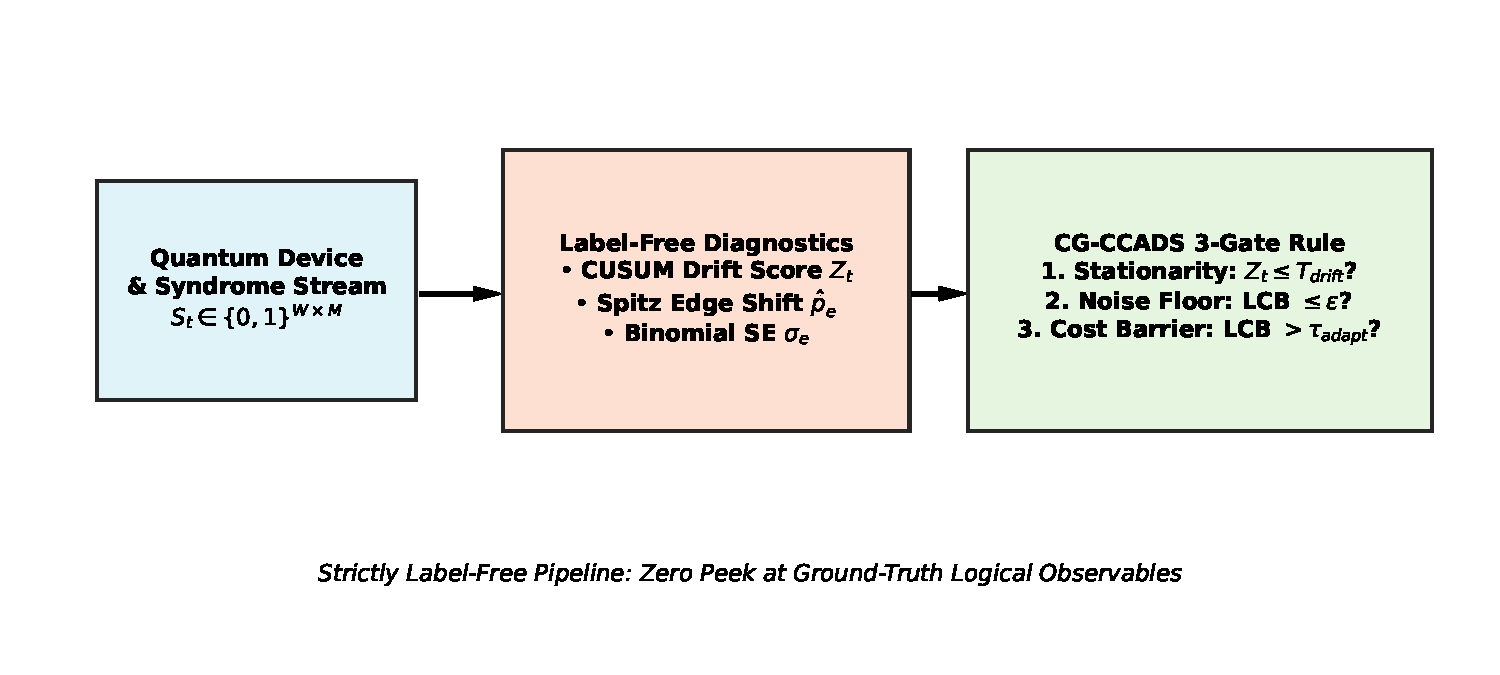
\includegraphics[width=0.95\textwidth]{figures/fig_2_architecture_diagram.pdf}
\caption{\textbf{CG-CCADS Architectural Pipeline.} The label-free syndrome stream is processed through three sequential statistical gates. When drift is absent or noise dominates (Gate 1 or 2), the controller enforces zero-cost abstention (\texttt{STAY}). Only when localized shifts exceed statistical confidence and amortized update taxes does the actuator commit graph reweighting.}
\label{fig:architecture}
\end{figure*}

\section{Related Work and Positioning}
Table~\ref{tab:prior_art} categorizes our framework relative to classical, neural, and adaptive decoding methodologies.

\begin{table*}[t]
\centering
\small
\caption{\textbf{Systematic Prior Art Comparison Matrix.} Positioning CG-CCADS within classical, neural, and adaptive QEC decoding frameworks.}
\label{tab:prior_art}
\begin{tabular}{lcccccc}
\toprule
\textbf{Framework} & \textbf{Noise Model} & \textbf{Adaptation Basis} & \textbf{Cost-Aware?} & \textbf{Safe Abstention (\texttt{STAY})?} & \textbf{Theoretical Bound} & \textbf{Evaluation Modality} \\
\midrule
Static MWPM~\cite{dennis2002,fowler2012} & Stationary Pauli & None (Fixed prior) & N/A & Always stays & Static threshold & Multi-platform QPU \\
Spitz et al.~\cite{spitz2018} & Time-dependent & Unconditional covariance & No & No & Estimator variance & Simulation \\
Bhardwaj et al.~\cite{bhardwaj2026} & Drifting channels & Sliding-window reweighting & No & No & Asymptotic convergence & Simulation \\
AlphaQubit~\cite{alphaqubit2024} & Device-calibrated & Transformer neural inference & No & No & Empirical scaling & Sycamore QPU \\
Willow RL~\cite{willow2026} & Physical Hamiltonian & Pulse/frequency tuning & Partial & No & RL Convergence & Willow QPU \\
\textbf{CG-CCADS (This Work)} & \textbf{Non-stationary QEC} & \textbf{3-Gate Statistical LCB} & \textbf{Yes} & \textbf{Yes (Default)} & \textbf{FWER-controlled LCB} & \textbf{Simulation / Emulation} \\
\bottomrule
\end{tabular}
\end{table*}


Spitz et al.~\cite{spitz2018} derived the fundamental covariance-parity relations enabling edge probability reconstruction from syndrome measurement coincidences without requiring logical state labels. Bhardwaj et al.~\cite{bhardwaj2026} demonstrated that updating MWPM edge weights in drifting superconducting channels reduces logical error under slow parameter variations. However, unconstrained online reweighting carries an implicit assumption that sample size is always sufficient to overcome finite-sample estimator variance. 

Our work bridges this gap. Rather than proposing a new decoding graph solver, we introduce a \textbf{decision-theoretic gating layer} that determines when to transition from a factory-calibrated prior to an online-reweighted model, preventing destructive updates during stationary or low-sample regimes.

\section{The Confidence-Gated Framework}

\subsection{Label-Free Covariance-Parity Estimator}
Following Spitz et al.~\cite{spitz2018}, consider a decoding graph $G = (V, E)$ where vertices represent detectors $u \in V$ and edges $(u, v) \in E$ represent independent fault mechanisms with error probability $p_{uv}$. For a window of $W$ binary syndrome measurement vectors $X \in \{0, 1\}^{W \times |V|}$, let $\bar{x}_u = \frac{1}{W} \sum_{k=1}^W X_{k, u}$ and $x_{uv} = \frac{1}{W} \sum_{k=1}^W X_{k, u} X_{k, v}$.
